\section{Detector Calibration}
\label{sec:calibration}
Calibration is extremely important to translating the response of the detector into the actually physical properties of an observed process.  The response of the SK detector to a particular physics process is essentially the combination of three responses:
\begin{itemize}
\item The physics of the initial process and production of photons through Cherenkov radiation
\item The propagation of photons through the water to the PMTs (water transparency)
\item  The response of the PMTs and electronics to the incident photons
\end{itemize}
Since the first response is what we are actually interested in observing, calibration is necessary to understand the second and third responses, so that we can translate the full detector response into an understanding of the actual physics process we are observing.  In this section I will discuss the main components of understanding the second two responses.  A detailed description of these and other aspects of detector calibration can be found in \cite{Abe:2013gga}.

\subsection{Water Transparency}
The propagation of photons through water is dictated by the equation:
\begin{equation}
I(l,\lambda)=I_0(\lambda)e^{\frac{l}{L(\lambda)}}
\label{eq:light_intensity}
\end{equation} 
 where $I(l,\lambda)$ is the intensity of light of wavelength $\lambda$ a distance $l$ from the source, $I_0(\lambda)$ is the initial intensity of the light, and $L(\lambda)$ is the total attenuation length at the given wavelength, which includes both scattering and absorption.  The attenuation length can be broken into three components:
\begin{equation}
L(\lambda)=\frac{1}{\alpha_{abs}(\lambda)+\alpha_{sym}(\lambda)+\alpha_{asy}(\lambda)}.
\end{equation}
Here $\alpha_{abs}(\lambda)$ is the absorption amplitude, $\alpha_{sym}(\lambda)$ is the ``symmetric" scattering amplitude, which is composed of Rayleigh scattering and symmetric Mie scattering, and $\alpha_{asy}(\lambda)$ is the ``asymmetric" scattering amplitude, which is composed of forward Mie scattering.  In order to measure these amplitudes, a collimated laser is injected at a few different wavelengths downward into the SK detector, as show in \cref{fig:laser}.  The detector is divided into seven regions, (top, bottom, five barrel regions), and the absorption and scattering amplitudes are tuned in MC so that the distribution of hits as a function a time in MC agrees with what is seen in data.  

\begin{figure}
\centering
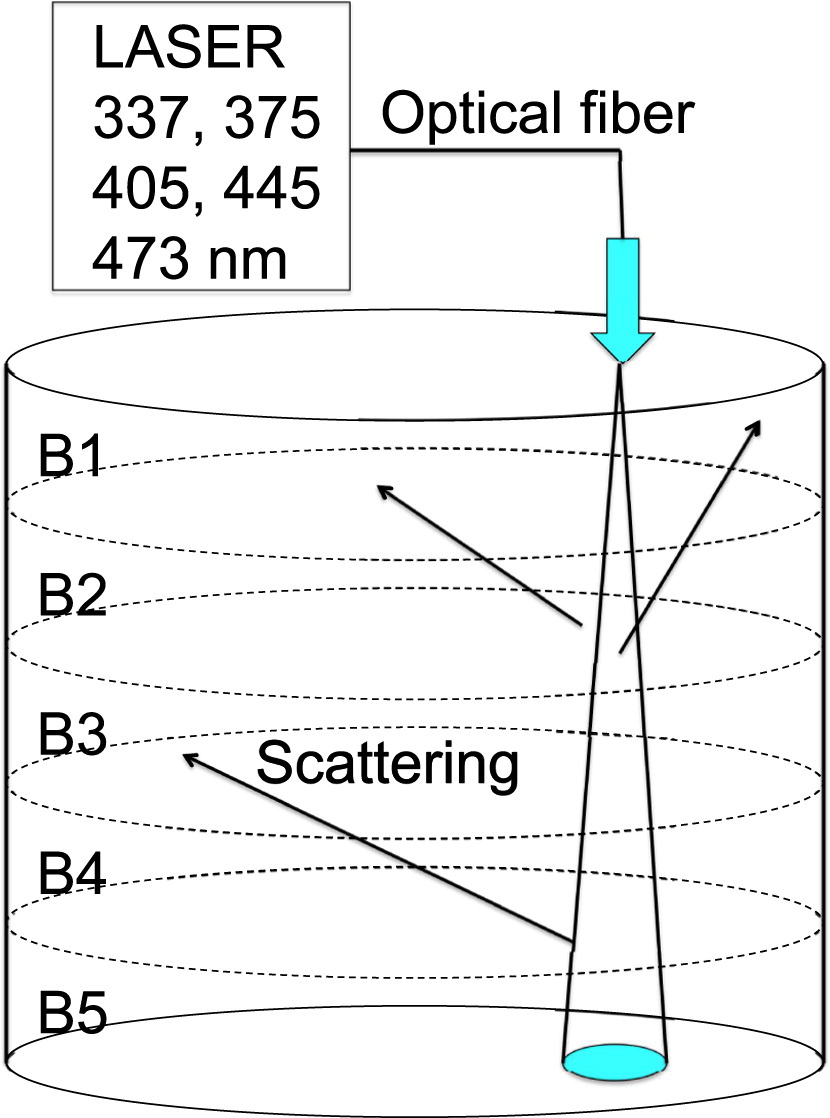
\includegraphics[width=0.5\textwidth]{figures/Laser.jpg}
\caption{Laser setup for water transparency measurement \cite{Abe:2013gga}.}
\label{fig:laser}
\end{figure}